% Activate the following line by filling in the right side. If for example the name of the root file is Main.tex, write
% "...root = Main.tex" if the chapter file is in the same directory, and "...root = ../Main.tex" if the chapter is in a subdirectory.
 
%!TEX root =  ../Thesis.tex

\chapter[Trigger and Cuts]{Trigger and Cuts}

The very first steps of any analysis consist of gathering the data, and then reducing the background
as much as possible.  For an experiment like ATLAS, with a dataset that approaches 3 PB of raw
data collected per year, picking a subset of that data for performing the search is both nontrivial
and crucial to the overall success of an analysis.  

The data selection starts with the trigger, which determines which events will even be recorded in the
first place.  The trigger must balance the competing forces of signal processes that can be very rare
(which would suggest a permissive trigger, so as to not lose already-rare signal events) and the
huge background rates at the LHC (which would suggest a strict trigger).  Since the trigger must make
decisions about event acceptance in near real-time, it can generally only require basic physics objects
like jets and $b$-tags, and more sophisticated background rejection gets implemented as offline event 
selection criteria, also called cuts.  

 
\section{Trigger}
\label{sec:my_trigger}
The purpose and structure of the ATLAS trigger are explained in Section~\ref{sec:atlas_trig}.
  The trigger chain for this analysis is as follows: 

\begin{itemize}
    \item L1: At least one J75 RoI (region of interest), implying an L1 jet of at least 75 GeV
    \item L2: least two 30 GeV jets, of which one must be at least 140 GeV. Additionally, at least two
jets must satisfy a medium b-tag (L2 xComb $>$ 1.276)
    \item EF: At least two 35 GeV jets, of which one must be at least 145 GeV. Additionally, at least two
jets must satisfy a medium b-tag (EF xComb $>$ 1.099). There is no explicit requirement that the
b-tagged jets from L2 correspond with the b-tagged jets from EF. However, as detailed later, this
requirement is added later as an offline cut.
\end{itemize}


In the trigger, the L2 and EF jets are b-tagged using xComb, a likelihood ratio of IP3D 
(significance of $z_0$ and $d_0$ impact parameters), SV1 (mass of the secondary vertex), NVTX (the number of
vertices with two tracks), and EVTX (the energy fraction of the secondary vertex), as well as the number
of vertices with 2 tracks. The triggers in this analysis use the medium operating point, such that L2 xComb
$>$ 1.276 and EF xComb $>$ 1.099.  This is the loose working point, where the $b$-jet efficiency
is 70\% online.

Table~\ref{tab:online_offline_btag} below shows the correlations between the two levels of online
$b$-tagging, as well as the offline (MV1) $b$-tagging for three offline working points (60\%, 70\%,
80\%).  

  \begin{table}[hbt]
\caption{  The acceptance of a cut on variable X given that the events have
  already passed (sig-like) or failed (bkgd-like) a cut on variable Y.\label{tab:online_offline_btag}}
    
    \begin{center}
    \begin{tabular}{l | l | c | c || c | c } \hline \hline
    \multicolumn{2}{c}{}  & \multicolumn{2}{c}{Signal MC} & \multicolumn{2}{c}{Unbiased Data} \\ \hline
      X         & Y         & sig-like & bkgd-like   &   sig-like & bkgd-like \\
      \hline
      EF        & L2        & 0.917    & 0.248 &   0.424       & 0.035 \\
      \hline
      L2        & MV1 (80)  & 0.675    & 0.031 &       0.510       & 0.077 \\
      EF        & MV1 (80)  & 0.824    & 0.090 & 0.515       & 0.050\\
      L2 and EF & MV1 (80)  & 0.676    & 0.036 & 0.414       & 0.031 \\
      MV1 (80)  & L2 and EF & 0.977    & 0.434 & 0.640       & 0.076 \\
      \hline
      L2        & MV1 (70)  & 0.716    & 0.060 & 0.652       & 0.086\\
      EF        & MV1 (70)  & 0.867    & 0.131 & 0.665       & 0.060 \\
      L2 and EF & MV1 (70)  & 0.721    & 0.060 & 0.563       & 0.038\\
      MV1 (70)  & L2 and EF & 0.954    & 0.340 & 0.538       & 0.034\\
      \hline
      L2        & MV1 (60)  & 0.757    & 0.101 & 0.762       & 0.095\\
      EF        & MV1 (60)  & 0.903    & 0.193 & 0.779       & 0.070 \\
      L2 and EF & MV1 (60)  & 0.765    & 0.103 & 0.692       & 0.045\\
      MV1 (60)  & L2 and EF & 0.902    & 0.250 & 0.429       & 0.015\\ \hline
    \end{tabular}
    \\
    \vspace{2mm}
    \end{center}
  \end{table}
  


%------------------------------------------------------
\begin{figure}
	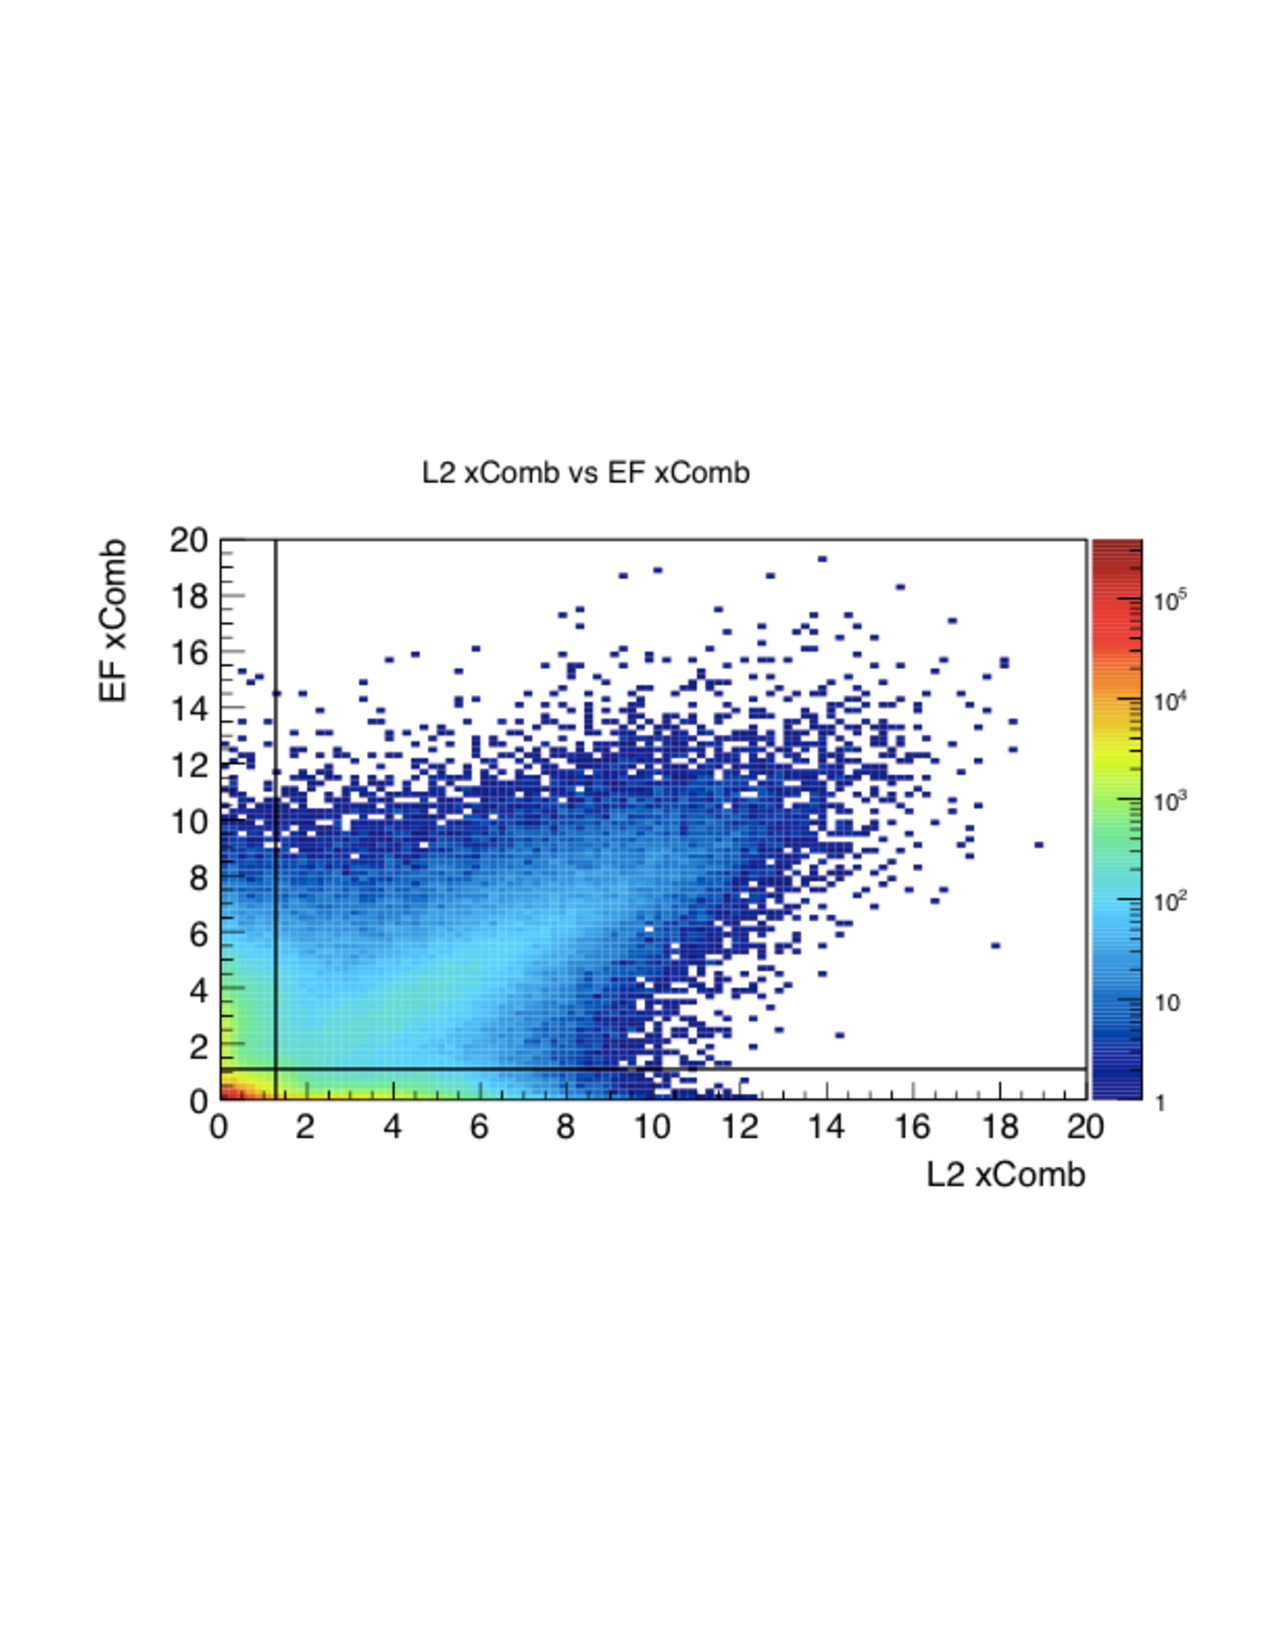
\includegraphics[width=0.6\textwidth]{TriggerCuts/L2_EF.pdf}	
    \caption{The cut efficiencies in background, cut by cut, shown on a linear (left) 
    and logarithmic (right) vertical axis. \label{fig:L2_EF}}
\end{figure}

%------------------------------------------------------
\begin{figure}
	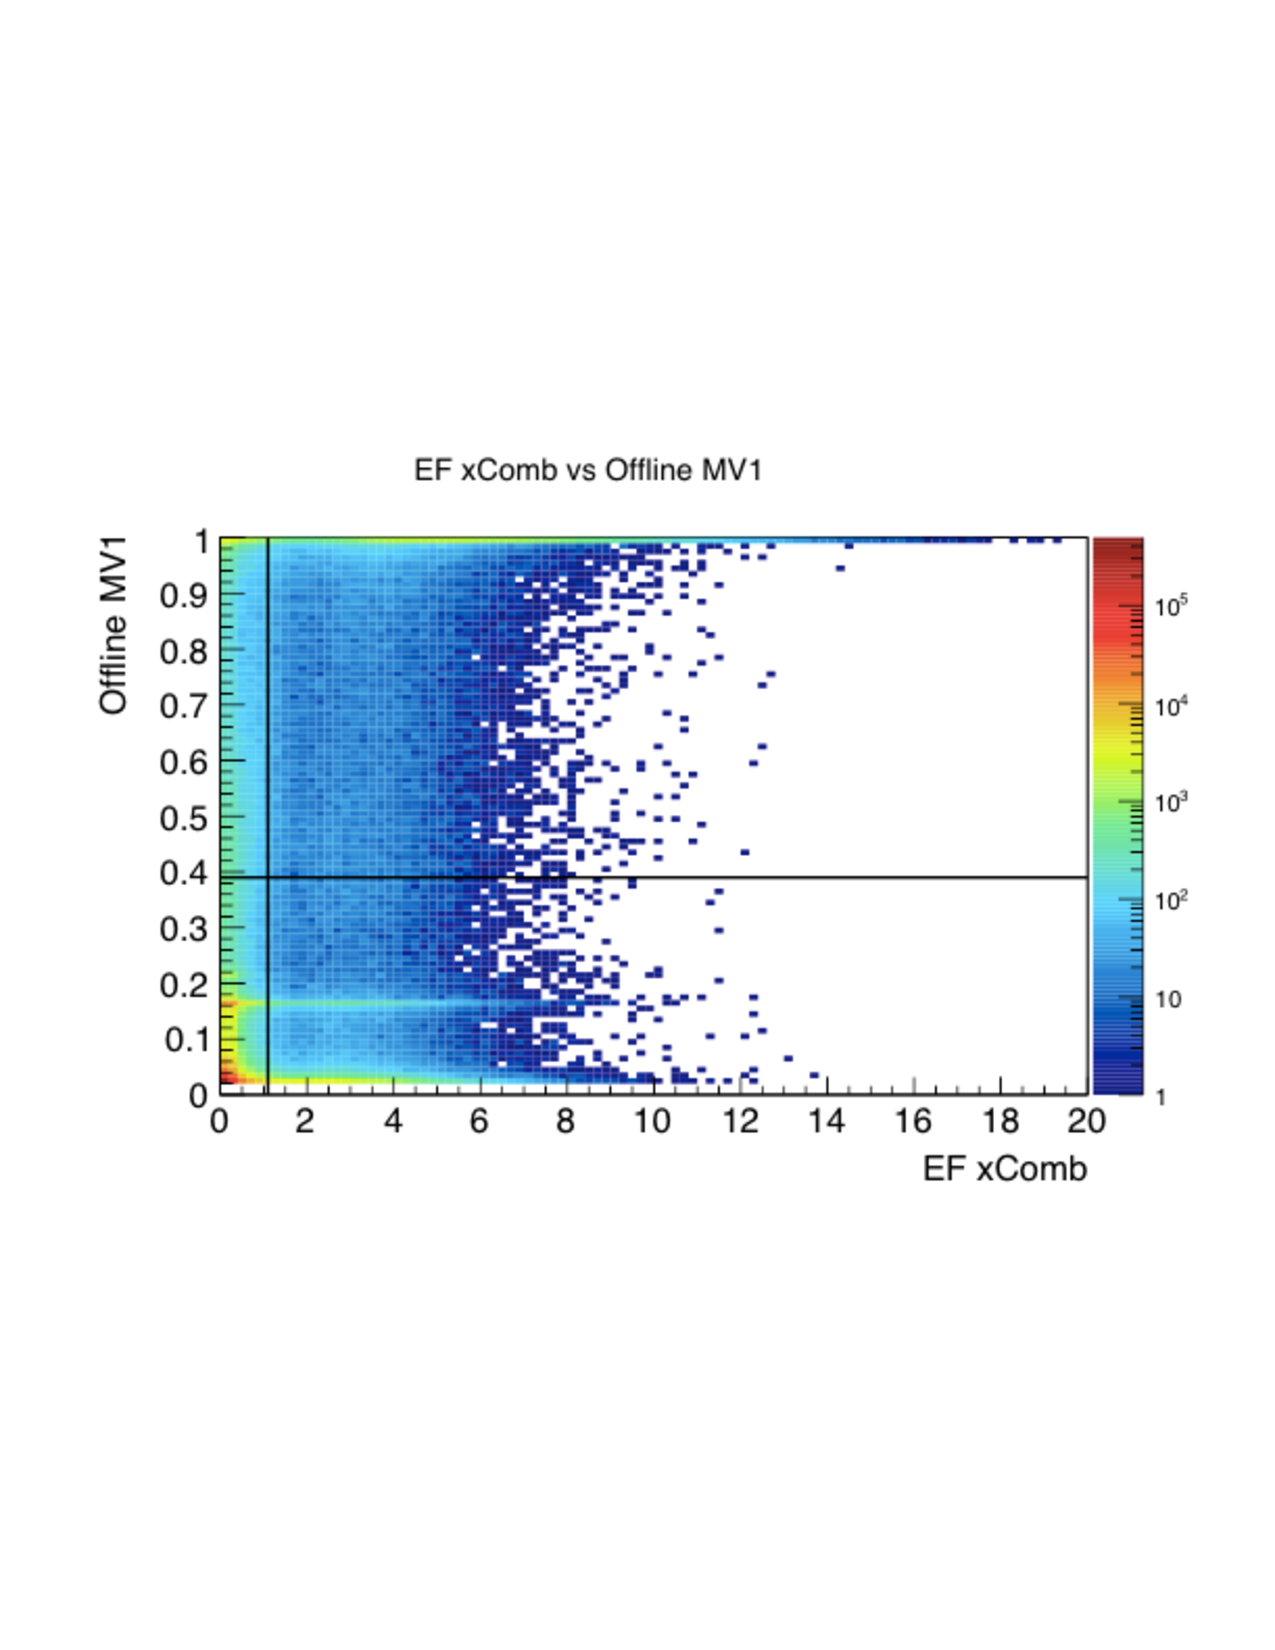
\includegraphics[width=0.6\textwidth]{TriggerCuts/EF_MV1.pdf}	
    \caption{The cut efficiencies in background, cut by cut, shown on a linear (left) 
    and logarithmic (right) vertical axis. \label{fig:EF_MV1}}
\end{figure}

%------------------------------------------------------










\section{Offline Baseline Cuts}


\begin{itemize}
\item
\textbf{$p_T$ cuts of 155 and 55 GeV on leading and sub-leading jets, respectively.}
In order to get out of the \pt turn-on curves of the trigger, cuts of
155~GeV and 55~GeV are applied to the leading and second jets in the
event.
\item
\textbf{$p_T$ cut of 25 GeV on third jet.}
A third jet is not required by the trigger, but is required by
the offline cuts, and it must have a \pt greater than 25 GeV.  There is
no veto on additional jets.  Further details on the jet cuts can be found
in Section~\ref{sec:jet_reco}.
\item
\textbf{Two jets passing online (L2 and EF in trigger) and offline (MV1) $b$-tags}
As part of the trigger, two jets are required to be $b$-tagged at L2 and at EF.  It
is not explicitly required by the trigger that the same jets pass $b$-tagging at the two trigger levels,
or that those jets be tagged offline by the MV1 algorithm, so we make an
offline cut that imposes that requirement.  There is further discussion of the online
and offline $b$-tagging correlations in Section~\ref{sec:online_btagging},
where one of the important conclusions is that there is not perfect correspondence
between jets passing the three levels of $b$-tagging (L2, EF, MV1).  For
example, a jet with a large xComb value at L2 (and passing the $b$-tagging
requirement at L2) might have a small xComb value at EF (and fail the $b$-tagging
requirement at EF).  Likewise with L2 and MV1, or EF and MV1.  As a result, we
make an explicit requirement offline that the same two jets be $b$-tagged in L2, EF
and MV1.  Jets that are tagged in both L2 and EF of the trigger are referred to as
``trigger-tagged'' jets, and jets that pass L2, EF and MV1 are called ``triple-tagged''
jets.
The offline cut on the
trigger-matched $b$-jets is set to the 60\% efficiency
operating point. Due to the bias introduced by the trigger (see
Table~\ref{tab:online_offline_btag}), this provides additional rejection of
light jets for a relatively small decrease in signal efficiency.


\item\textbf{Leading 2 jets must pass tight MV1 $b$-tag}
It is also required that the two jets in the event with the highest \pt be $b$-tagged
offline by the MV1 algorithm.  There is no explicit requirement that the leading
two jets be trigger-tagged or triple-tagged.
  In addition to preferentially keeping signal events at a higher rate than
background events, this cut considerably improves the combinatorics of reconstructing
the Higgs and we see markedly better signal mass peak resolution when this cut is in
place.  Further details can be found in Section~\ref{sec:combinatorics}.


\item
\textbf{Third jet passing offline $b$-tag}
After two
$b$-jets have been triple-tagged, a third jet is tagged using the MV1 tagger.  The third
$b$-jet must have an MV1 value that passes a tight (60\% efficiency)
cut.  The light-jet efficiency for this working point is approximately 0.1\%, and the
charm efficiency is approximately 10\%.

\end{itemize}



%------------------------------------------------------
\begin{figure}
	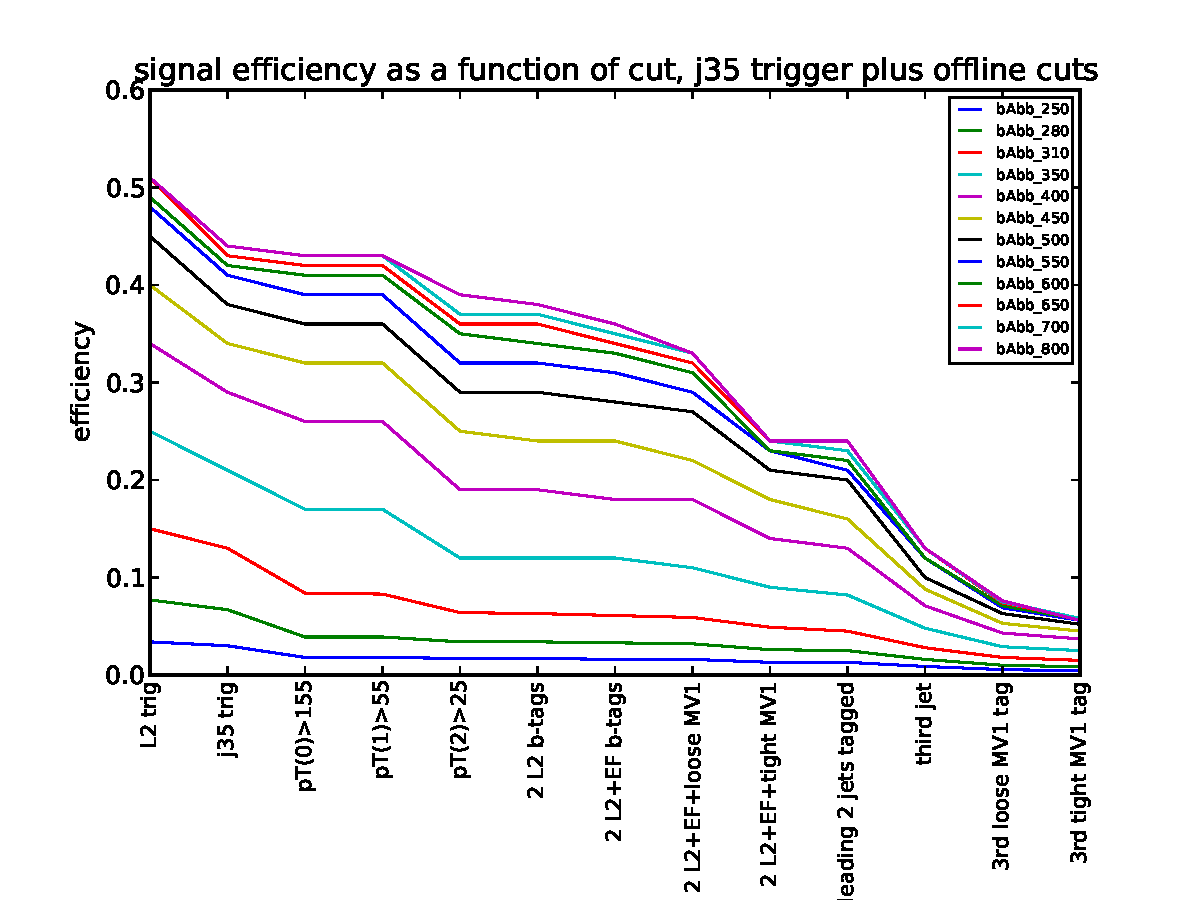
\includegraphics[width=0.4\textwidth]{TriggerCuts/cut_efficiencies_j35_signal.pdf}	
	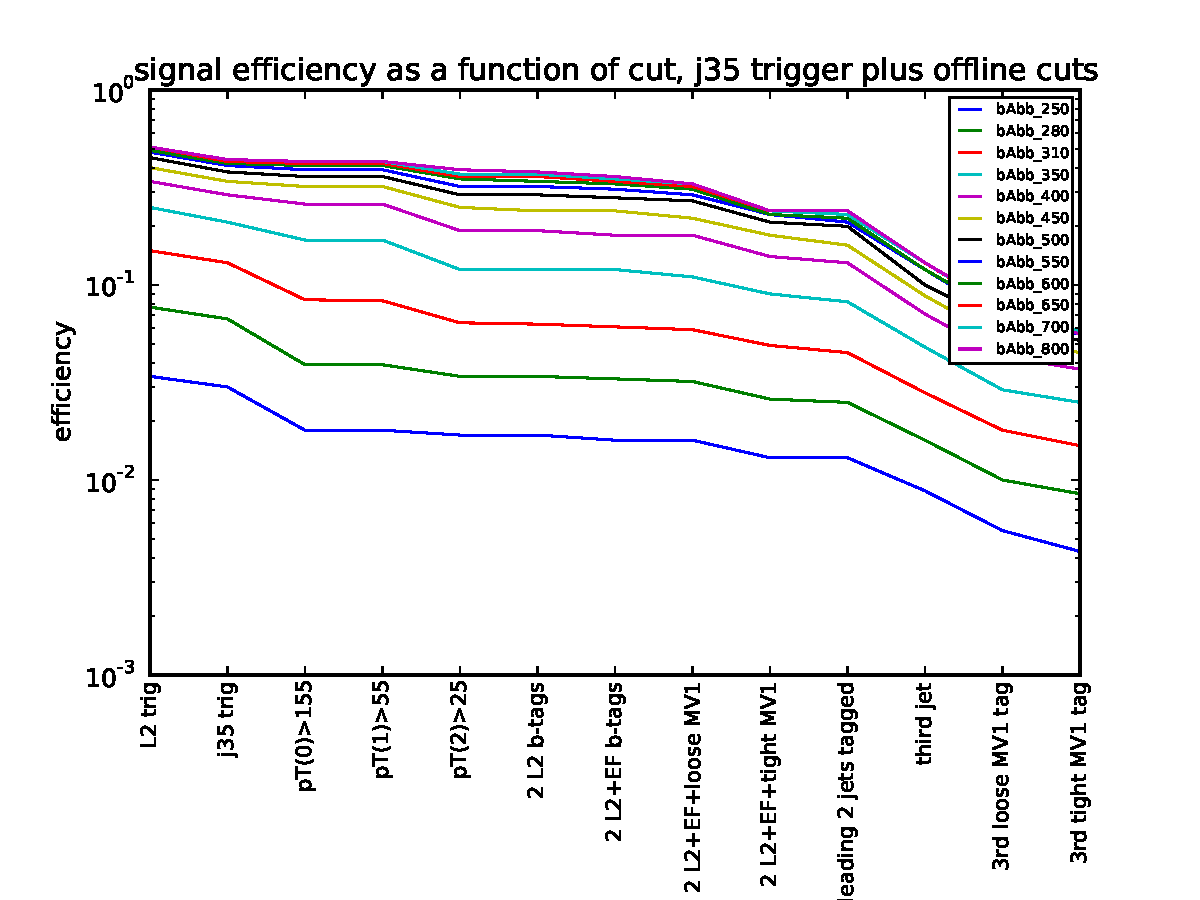
\includegraphics[width=0.4\textwidth]{TriggerCuts/cut_efficiencies_logy_j35_signal.pdf}	
    \caption{The cut efficiencies in signal, cut by cut, shown on a linear (left) and logarithmic (right) vertical axis. \label{fig:signal_eff_cutflow}}
\end{figure}

%------------------------------------------------------





%------------------------------------------------------
\begin{figure}
	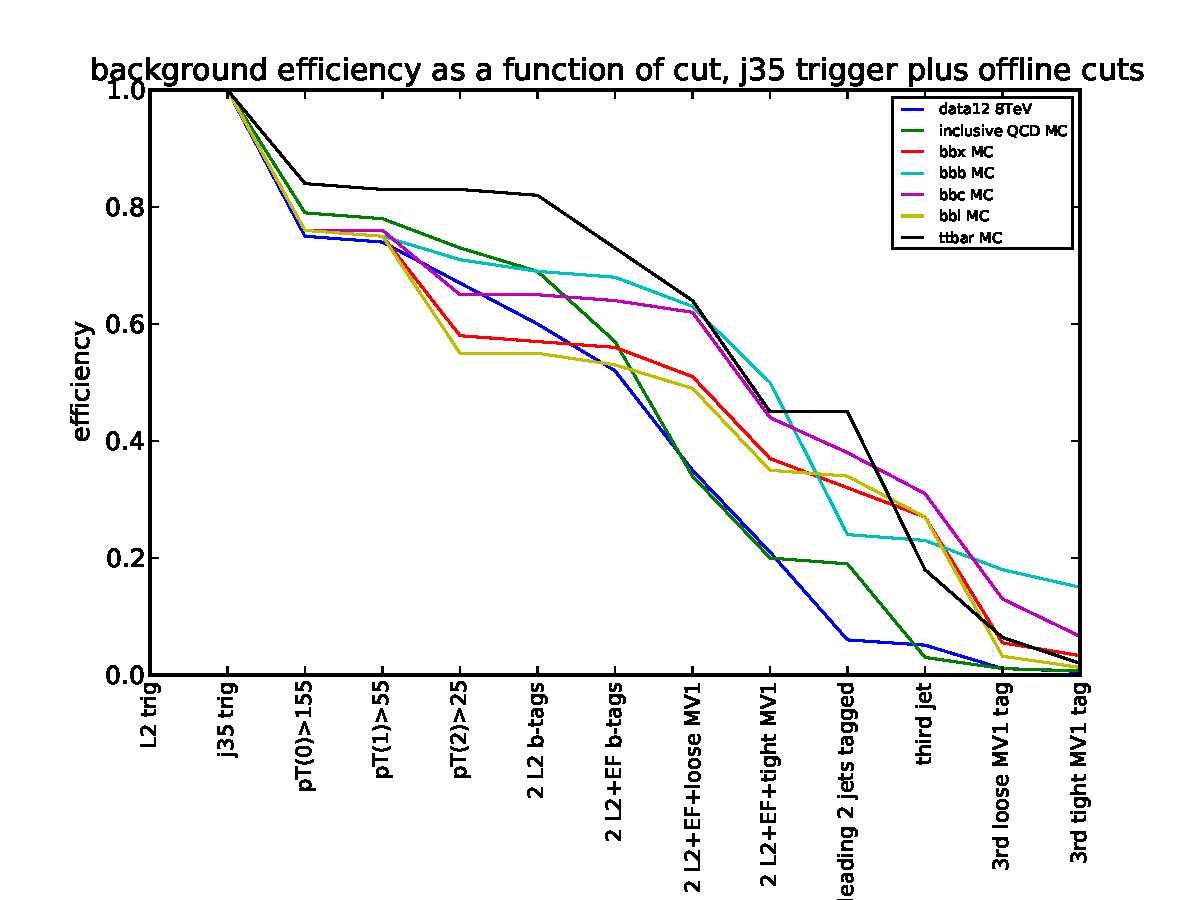
\includegraphics[width=0.4\textwidth]{TriggerCuts/cut_efficiencies_j35_background.pdf}	
	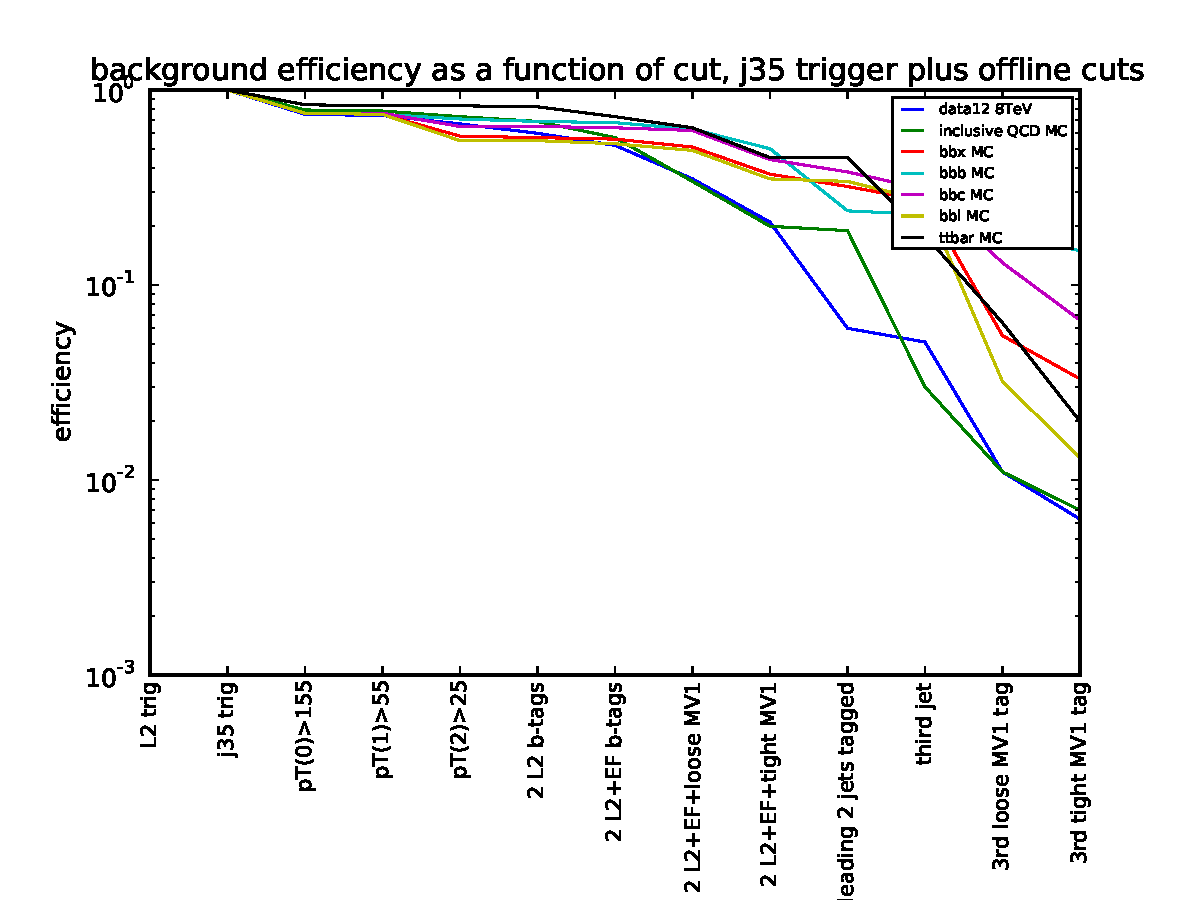
\includegraphics[width=0.4\textwidth]{TriggerCuts/cut_efficiencies_logy_j35_background.pdf}	
    \caption{The cut efficiencies in background, cut by cut, shown on a linear (left) and logarithmic (right) vertical axis. \label{fig:background_eff_cutflow}}
\end{figure}

%------------------------------------------------------

%------------------------------------------------------
\begin{figure}
	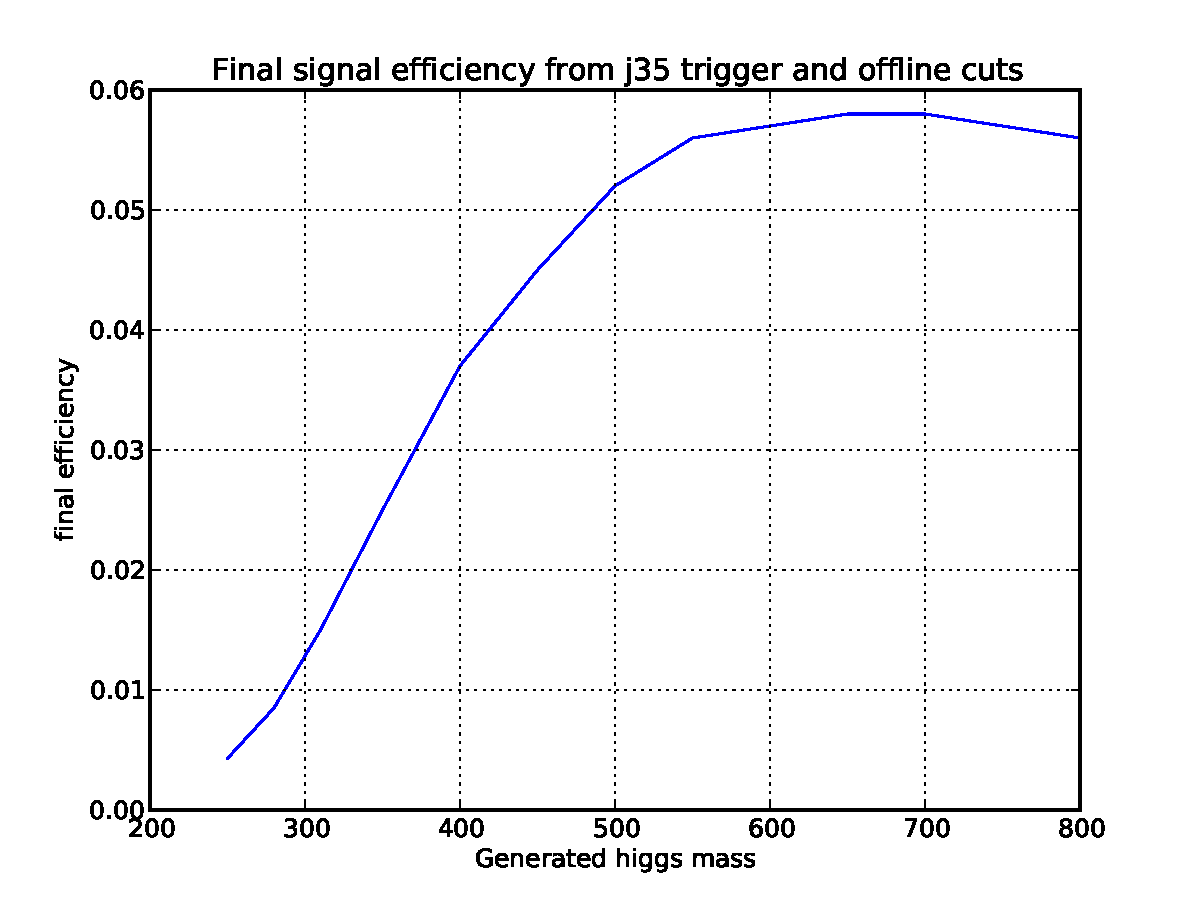
\includegraphics[width=0.6\textwidth]{TriggerCuts/final_efficiency_vs_mass_j35.pdf}	
    \caption{The cut efficiencies in background, cut by cut, shown on a linear (left) and logarithmic (right) vertical axis. \label{fig:final_eff_vs_mass}}
\end{figure}

%------------------------------------------------------







